%!TEX root = ../main.tex

\chapter{Tire-Ground Enveloping Modeling}
\label{app2:enve}

As previously introduced in Appendix~\ref{app1:acme}, simulation has become vital in vehicle development and virtual testing, especially for autonomous vehicles. High-performance \ac{HRT} simulators, which are crucial for those undertakings, require efficient algorithms to accurately model vehicle behavior within virtual environments. A prime example is tire-ground contact modeling, which is pivotal if we aim to achieve a high level of realism when simulating wheeled vehicles. Contact modeling focuses on an accurate estimation of the parameters needed to compute the forces and torques generated by vehicle-ground interaction. However, the complexity of this task is compounded by the fact that tire-ground contact is a highly non-linear phenomenon, which is further exacerbated by the need to perform tests to fine-tune state-of-the-art tire-ground contact models. To tackle those challenges, we have developed a novel enveloping model that does not require any fitting of experimental data and is based on the 3D geometry of the intersection between undeformed volumes. In this appendix, we provide a detailed description of the algorithm's formulation, the current software implementation, which is available as a BSD-3-Clause open-source library under the name \Enve{}, as well as the achieved scalability and \ac{RT} performance.

% % % % % % % % % % % % % % % % % % % % % % % % % % % % % % % % % % % % % % % %

\section{Introduction to Tire-Ground Contact Modeling}
\label{app2:sec:introduction}

From the 1950s onwards, vehicle simulation has been crucial for evaluating ride and handling. More recently, as we shift towards autonomous vehicles, there's a growing need for high-quality simulations to develop and test them in various scenarios. Real-world testing is time-consuming and costly, making driving simulators essential for accelerating the transition to autonomous driving, enhancing safety, and reducing expenses. Beyond the hardware, a simulator's essence lies in its software, responsible for shaping the virtual environment based on physics. Aside from computer graphics, this software comprises multiple subprograms, including a \ac{MBS} -- used to integrate the \ac{MB} car system -- and several other subprograms that allow the \ac{MB} system to interact with the environment. In the case of a road vehicle, interactions with the environment primarily occur through tire-ground contact, aerodynamic forces, and, less frequently, through collisions with external objects. To obtain a sufficiently realistic simulation of the vehicle it is therefore of crucial importance to correctly estimate the forces and torques generated by the tire-ground contact~\cite{pacejka2012tire}. In order to be able to calculate the stress generated by the contact, the first step is to estimate the ground rut pose with respect to the tire reference frame~\cite{pacejka2005spin}. An incorrect estimate of the \emph{local contact plane} or \emph{surface} would inevitably lead to unrealistic or unreliable simulations. Since tire-ground contact evaluation is one of the most time-consuming processes in \ac{MB} simulations, algorithms designed specifically for this purpose are needed to ensure high efficiency and scalability. Specifically, in the case of \ac{DIL}, \ac{HIL}, and/or \ac{SIL} simulations, this software must guarantee a capability that is at least as fast as \ac{RT}. It is also desirable to obtain a faster than \ac{RT} capability, in order to speed up costly offline simulations and to allow for the use of less powerful machines.  As a matter of fact, the development of faster and at the same time more accurate contact models still remains an open research topic~\cite{gallrein2014advanced, serban2023realtime}.

From the scientific literature, it is known that appropriate contact methods must be applied when road unevenness is characterized by wavelengths 2--3 times smaller than the contact patch length. This occurs when riding is done either over cobblestone or Belgian block roads, or simply over road surfaces that present sharp obstacles, \eg{}, cleats, bumps or potholes~\cite{pacejka2012tire}. The role of the tire-ground contact model is to represent the excitation of pneumatic tires caused by uneven terrain surfaces. Although the term ``uneven ground surface'' comprehends any kind of unevenness, attention is mainly paid to short irregularities, as tire deformation is particularly important in those instances. The ability of the tire to deform, \ie{}, to follow the ground surface shape, is defined as the \emph{enveloping} property of the tire-ground contact. In specific, the enveloping is the \emph{quasi-static} component of the tire-ground contact phenomenon, whereas the \emph{dynamic} component comes from the carcass flexibility and is implemented in the tire force-calculation model~\cite{pacejka2012tire, schmeitz2004semiempirical}. The enveloping property depends on the tire geometry and structure, and can be represented through \emph{physical} models such as those presented in~\cite{davis1975radial, badalamenti1988radial, negrut1994dynamic, mousseau2003obstacle, kim2008two}, or (\emph{semi-})\emph{empirical} models such as~\cite{rill2013tmeasy, schmeitz2004semiempirical}. In contrast to physical models, the empirical models try to describe the contact through much simpler models designed to mimic the behavior of the tire-ground interaction.

In the early days of vehicle simulation, studies on tire behavior have mostly been limited to the case of flat and asperity-free contact surfaces, focusing on the deformation and dynamics of the tire carcass induced by the contact forces. The importance of accurately describing the local contact area has been highlighted in~\cite{kageyama2002study, pacejka2005spin}, where the influence of obstacles on the overall tire behavior is studied. While the tire is riding over 3D uneven road surfaces the local road plane shows variations in height, and in forward and banking angles. The banking slope angle gives rise to the so-called tire camber thrust, which must be taken into account in order to properly simulate the force generated by the tire. Since then, many enveloping models for arbitrarily uneven surfaces have been developed. Most of the models developed so far are based on heuristic concepts. Without a doubt, the most famous enveloping model is certainly the \Swift{} model, which allows the \ac{MF} model to be used even on rough road surfaces~\cite{schmeitz2004semiempirical}. Simple and parameterless contact models like that used in \TMEasy{}~\cite{rill2013tmeasy, rill2018sophisticated} can be applied, but do not always guarantee adequate enveloping properties,  which can cause sudden and unrealistic variations of the banking and slope angles in the proximity of sharp cleats or asperities. Another family of more sophisticated enveloping models is based on the physical concept of radial and radial-interradial spring tire~\cite{davis1975radial, badalamenti1988radial, negrut1994dynamic}. Models based on the tire radial-spring behavior are a good compromise between computational effort, robustness and physical consistency. Unlike the \Swift{} model, the radial spring tire models do not show any working range limit in shape, magnitude and orientation of the incoming road obstacles~\cite{davis1975radial}. For this reason, the results are physically consistent even in the case of high cleats. The state-of-the-art approach is referred to as ``full-physical tire modeling''. In particular, the commercial software \FTire{}~\cite{gipser2005ftire} and \CDTire{}~\cite{gallrein2007cdtire, gallrein2014advanced} are the leading virtual tire simulation models in this category. They are proven to be multi-purpose physics-based tire models that are able to simulate nearly all tire dynamics phenomena. They combine a discrete elements description of both belt and sidewalls elements with a brush type contact, and \ac{RT} capabilities~\cite{gipser2021ftire}. In terms of enveloping behavior, they are also providing physically consistent and extremely realistic results~\cite{gipser2008ftire, gallrein2007cdtire}. Unfortunately, little information on the actual computational time performance is available for both \FTire{} and \CDTire{}.

A very simple physical contact modeling approach we have not yet mentioned before relies on the geometry of intersection between undeformed regions, also known as displaced area models~\cite{mousseau2003obstacle}. This kind of model is derived from the physics of the linear radial-spring tire model. As stated also in~\cite{davis1975radial} a common approach for modeling the 2D vehicle-road contact is to assume that the tire is described by a disk moving on a ground region. Indeed, if we assume that the tire is represented by an infinite number of independent linear radial springs, the force resulting from the contact is linearly proportional to the intersection area and acts along the line passing through the centroid of the intersection region and the wheel center. Despite the simplicity of this approach and the limits that arise from neglecting the tire carcass being a unique cohesive body capable of transmitting shear forces, it provides a good approximation of the contact information. Models based on the geometry of intersection between undeformed regions are already available, but they all lack a full 3D description of the contact. This limits the comparison between other enveloping models to 2D contact scenarios. Moreover, no robust software implementation is freely available and can be used to determine the tire contact point and normal or equivalently a contact plane.

This appendix aims to present a software-based algorithm (hereafter called \Enve{}) to model the 3D geometrical contact between tire and ground, represented respectively as a generic axial-symmetric surface and a triangular mesh. In particular, the adopted methodology is derived from the physics of the linear radial-spring tire model and is based on the geometry of the intersection between undeformed regions. Indeed, \Enve{} is an enveloping model that is fully parameterizable by the tire's external shape alone and does not require any fitting on experimental data. As will be shown in the following, the proposed approach achieves an efficient and robust modeling of the tire-ground geometrical contact with scalable precision. This model is intended to be coupled with a tire model, \ie{}, empirical or physical tire model, with or without belt and sidewall dynamics. The tire model calculates tire-ground forces based on geometric contact parameters supplied by the \Enve{} software. In this study, we demonstrate the efficiency and efficacy of the software by coupling \Enve{} with the \ac{MF}~6.2 tire model.
%
\begin{remark}
  In this appendix, the focus will only be on the enveloping properties of the tire-ground contact, \ie{}, the calculation of the so-called effective road surface. To evaluate dynamic response, one can employ a rigid ring model coupled with a tire model for force calculation, as exemplified by \ac{MF}-\Swift{}~\cite{pacejka2012tire, schmeitz2004semiempirical}. In this appendix, our aim is to determine the application point and direction of contact forces, and as such, we do not delve into the modeling of tire-ground contact forces or the tire carcass dynamics.
\end{remark}
%
This appendix has two main goals. The first is to provide a methodology for the analysis of the geometrical tire-ground contact, which takes into account the geometry of the tire cross-section and of the road surface to compute information needed by the tire model to obtain forces. The proposed enveloping model offers advantages over \Swift{} in terms of algorithm simplicity and scalability. It excels in computing contact on multiple sections, making it suitable for supporting physical-based tire models like the brush model. Additionally, it does not rely on independently identified parameters, further enhancing its effectiveness and immediacy of use. These characteristics make it suitable for \ac{HRT} applications where computational efficiency is the main concern without diminishing the level of accuracy. The second is to evaluate the impact of this new approach coupled with a tire model in an advanced simulation environment with \ac{HRT} scheduling. The software, which is also called \Enve{}, is built on the \Acme{} geometry library (see Appendix~\ref{app1:acme} or \citet{stocco2021acme}), and is designed to be integrated into vehicle dynamics \ac{MB} kernel codes as well as into simpler simulation environments~\cite{piccinini2022predictive, piccinini2023physics}.

% % % % % % % % % % % % % % % % % % % % % % % % % % % % % % % % % % % % % % % %

\section{Tire-Ground Enveloping Model}
\label{app2:sec:model}

Let us consider a reference frame $\pt{H}xyz$ with unit vectors ($\et{h}_x$, $\et{h}_y$, $\et{h}_z$), whose origin $\pt{H}$ is located in the wheel hub (see \figurename{}~\ref{app2:fig:tire_shell}). The axes are oriented according to the ISO 8855:2011 standard~\cite{iso88552011}. The $x$-axis is directed towards the longitudinal direction of motion, the $z$-axis points upwards and the $y$-axis is oriented in such a way that the coordinate system is right-handed. The tire is defined geometrically as an axially symmetric (around the axis $\et{h}_y$), convex and closed set $\sett{T}$
%
\begin{equation}
  \sett{T} = \big\{ [x, y, z]^\mathrm{T} \in \mathbb{R}^3, ~ y \in [ y_l, \, y_r ], ~ R(y):\mathbb{R} \mapsto \mathbb{R}_{\geq 0} ~ \big\lvert ~ \sqrt{x^2+z^2} \leq R(y) \big\}  \, \text{,}
\end{equation}
%
whose interior and boundary are respectively denoted with $\interior{T}$ and $\boundary{T}$. The function $R(y)$ can be chosen arbitrarily to properly reconstruct the tire's external morphology. On the other hand, the ground is modeled as a closed half-space $\sett{G}$
%
\begin{equation}
  \sett{G} = \big\{ [x, y, z]^\mathrm{T} \in \mathbb{R}^3 ~ \big\lvert ~ z \leq g(x,y), ~ g(x,y): \mathbb{R}^2 \mapsto \mathbb{R}, ~ f(x,y):\mathbb{R}^2 \mapsto \mathbb{R}_{\geq 0}\big\}  \, \text{,}
\end{equation}
%
whose interior and boundary are respectively denoted with $\interior{G}$ and $\boundary{G}$. The map $g(x,y)$ is a mapping between $\mathbb{R}^2$ to $\mathbb{R}$ that defines the height of the track surface. Similarly, the map $f(x,y)$ defines the local friction coefficient scaling factor, which is used to scale the tire performance according to the local ground surface conditions. Notice that the concept behind the friction coefficient scaling factor can be extended to other relevant local properties of the ground surface, \eg{}, temperature, water film thickness, and asphalt wear.

\begin{figure}
  \begin{subfigure}[t]{0.475\textwidth}
    \centering
    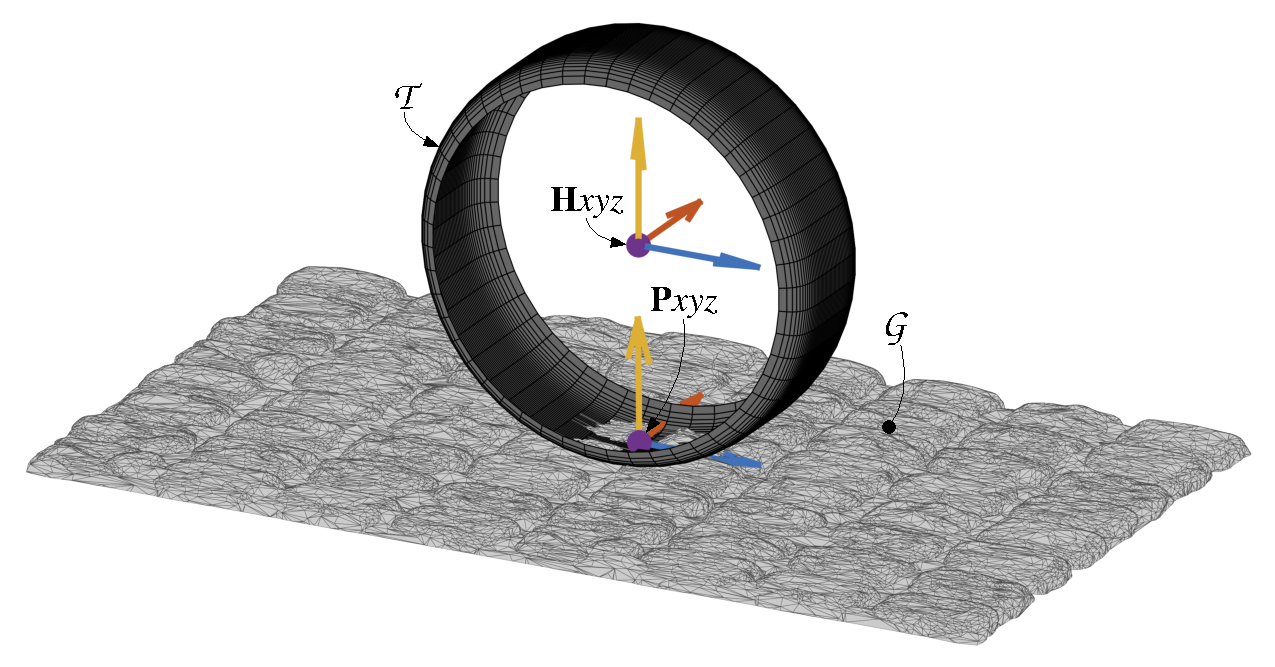
\includegraphics[width=1.0\textwidth, trim={5cm 2.3cm 5cm 0cm}, clip]{./figures/appendix_2/road_shell_ipe}
    \caption{Representation of the intersection between the tire $\sett{T}$ and a Belgian block road boundary $\sett{G}$ alongside the hub $\pt{H}xyz$ and the contact point $\pt{P}xyz$ reference frames.}
    \label{app2:fig:tire_shell}
  \end{subfigure}
  \hfill%
  \begin{subfigure}[t]{0.475\textwidth}
    \centering
    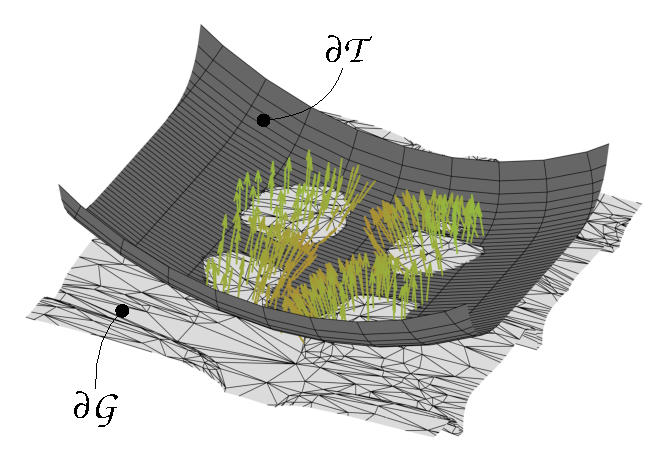
\includegraphics[width=1.0\textwidth]{./figures/appendix_2/zoom_ipe}
    \caption{Representation of the ground boundary $\boundary{G}$ normal directions (green arrows) inside the tire set boundary $\boundary{T}$. Each of these directions, together with other information, is exploited to calculate the contact point $\pt{P}$ and normal $\et{n}$.}
    \label{app2:fig:zoom}
  \end{subfigure}
  \caption{Representation of the tire-ground contact.}
  \label{app2:fig:tire_ground}
\end{figure}

To identify and quantify the contact between the tire and the ground we need to define what the intersection volume and the contact patch regions are. The intersection region is a closed set $\sett{V}$, collecting all the points of the tire $\sett{T}$, which are also points of the ground set $\sett{G}$, \ie{}, $\sett{V} = \sett{T} \cap \sett{G}$ (see \figurename{}~\ref{app2:fig:zoom}). On the other hand, the contact patch is defined as a closed set $\sett{P}$ that collects all the points of the tire which are also interior points of the ground boundary surface $\boundary{G}$, \ie{}, $\sett{P} = \sett{T} \cap \boundary{G}$. The contact area $A$ and the contact volume $V$ are defined respectively as
%
\begin{center}
  \begin{minipage}[b]{0.425\textwidth}
    \vspace{-\baselineskip}
    \begin{equation}
      A = \iint_\sett{P} 1 \, \de\sett{\pt{x}}  \, \text{,}
      \label{app2:eq:int_area}
    \end{equation}
  \end{minipage}%
  \hfill\hfill and \hfill
  \begin{minipage}[b]{0.425\textwidth}
    \vspace{-\baselineskip}
    \begin{equation}
      V = \iiint_\sett{V} 1 \, \de\sett{\pt{x}} \, \text{.}
      \label{app2:eq:int_volume}
    \end{equation}
  \end{minipage}
\end{center}

The tire is assumed to be modeled by an infinite number of \emph{independent linear radial-springs}, whose stiffness $k$ is uniform all over the tire section. The inaccuracy introduced by this assumption is recovered by the tire force-calculation model, which employs concentrated parameters to describe the non-uniformity of the carcass stiffness. Before calculating the direction $\et{n}$ and application point $\pt{P}$ of the resultant contact force, we have to make three important observations.

\begin{observation}
  The force generated by the contact is produced by the deformation of the radial springs. If the terrain is non-deformable the contact force magnitude $\|\vt{F}\|$ is linearly proportional to the intersection volume $V$, \ie{},
  %
  \begin{equation*}
    \| \vt{F} \| = \iiint_\sett{V} k \, \de\sett{\pt{x}} = k V \propto V \, \text{.}
  \end{equation*}
  %
\end{observation}
%
Notice that the proportionality constant is the stiffness coefficient $k$, which is a function of the tire's internal structure and pressure. However, these dependencies are considered by the tire force-calculation model through lumped parameters. It should be pointed out that the damping effect is not considered due to the quasi-static nature of the enveloping phenomenon.
%
\begin{observation}
  Since the tire is assumed to be modeled by an infinite number of independent radial springs, the contact force $\vt{F}$ cannot produce any rolling resistance torque around the wheel hub axis $\et{h}_y$. In other words, the contact force acts along the direction determined by one of the families of lines passing through the contact point $\pt{P}$ and the hub axis $\et{h}_y$.
\end{observation}
%
It is also important to note that the rolling resistance is not considered in the enveloping models. It is typically considered to be part of the tire contact force model, which must be fed with the information provided by the enveloping model. For instance, the \Swift{} model is coupled with the \ac{MF} model to compute the contact forces and torques generated by the tire-ground contact.

Thanks to these observations, the duality between the physical and geometrical models of the tire-ground contact can be exploited. Hence, the contact point $\pt{P}$ is calculated as the weighted average of contact surface points. The weight is proportional to the infinitesimal radial volume interested in the tire-ground contact. This infinitesimal radial volume is calculated as the intersection of the contact volume with the line $\ell(\pt{x},\et{h}_y)$ passing through the point $\pt{x} = [x, \, y, \, x]^\mathrm{T}$ and matching the axes of the wheel $\et{h}_y$ orthogonally. If $\mathrm{proj}(\pt{x},\boundary{G})$ defines the intersection point of the line $\ell(\pt{x},\et{h}_y)$ with $\boundary{G}$, then $\pt{P}$ is calculated as
%
\begin{equation}
  \pt{P} = \dfrac{1}{V} \displaystyle\iiint_\sett{V} \mathrm{proj}(\pt{x},\boundary{G}) \, \de\sett{\pt{x}}
  \, \text{.}
  \label{app2:eq:int_p}
\end{equation}
%
The application direction of the resultant tire-ground contact force is denoted by $\et{n}$. It is calculated as the average of the directions $\et{d}(\pt{x},\et{h}_y)$ of the lines $\ell(\pt{x},\et{h}_y)$, \ie{},
%
\begin{equation}
  \vt{n} = \displaystyle\iiint_\sett{V} \et{d}(\pt{x},\et{h}_y) \, \de\sett{\pt{x}},
  \qquad \text{where} \qquad
  \et{n} = \dfrac{\vt{n}}{\|\vt{n}\|}
  \, \text{.}
  \label{app2:eq:int_n}
\end{equation}
%
Similarly, the overall tire friction coefficient scaling factor $\lambda$ is calculated as
%
\begin{equation}
  \lambda = \dfrac{1}{V} \displaystyle\iiint_\sett{V} f(\pt{x}) \, \de\sett{\pt{x}}
  \, \text{.}
  \label{app2:eq:int_l}
\end{equation}
%
The solution of the here defined integrals~\eqref{app2:eq:int_p}, \eqref{app2:eq:int_n}, and~\eqref{app2:eq:int_l} is not straightforward. This is why, in the next section, we propose a numerical approximation of these integrals.

It should be pointed out that the local ground plane is hereafter identified by the reference frame $\pt{P}xyz$ whose origin point is $\pt{P}$ and axes directions are
%
\begin{align*}
  \et{e}_z = \et{n} \, \text{,} \quad
  \et{e}_x = \dfrac{\et{h}_y \times \et{n}}{\|\et{h}_y \times \et{n}\|} \, \text{,} \quad \text{and} \quad
  \et{e}_y = \et{n} \times \et{e}_x
  \, \text{.}
\end{align*}
%
The $\beta_x$ and $\beta_y$ angles, which are used to describe the local ground surface orientation with respect to the wheel hub, are calculated as the Euler angles ($zxy$ sequence) between the hub reference frame $\pt{H}xyz$ and the contact point reference frame $\pt{P}xyz$ (see \figurename{}~\ref{app2:fig:tire_iso}).

\begin{figure}[!htb]
  \centering
  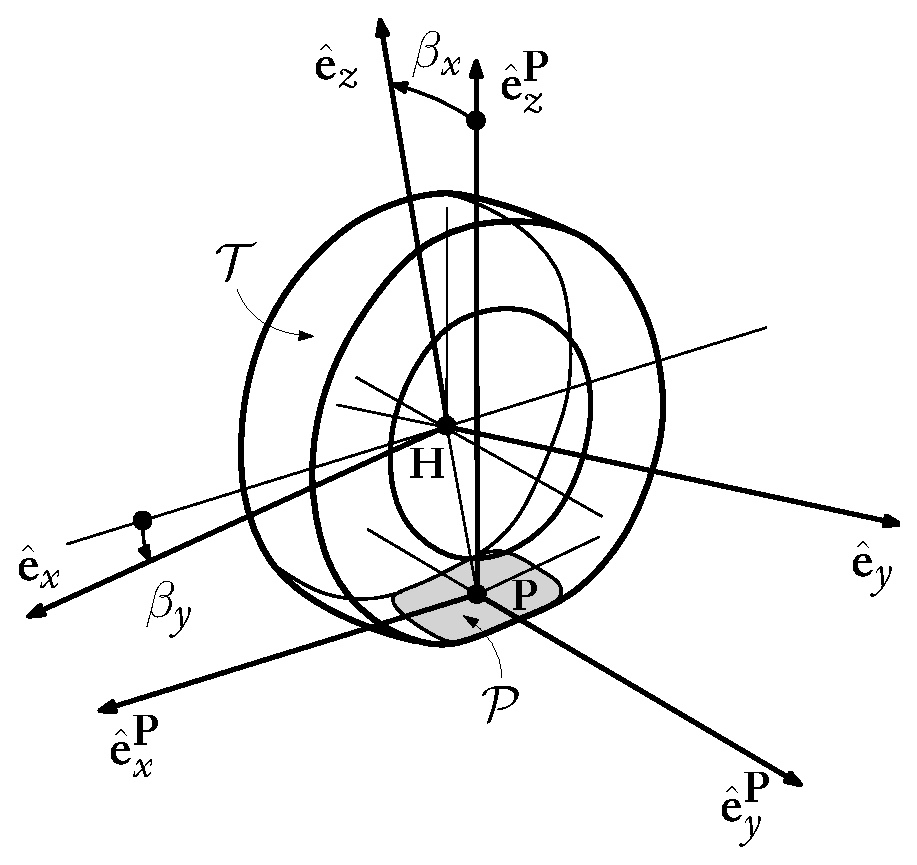
\includegraphics[width=0.5\textwidth]{./figures/appendix_2/tire_iso}
  \caption{Representation of the contact pose $\pt{P}xyz$ along with the hub reference frame $\pt{H}xyz$ according to the ISO standard~\cite{iso88552011}. The constant pose is defined by the contact point $\pt{P}$ and the normal $\et{e}_z = \et{n}$, which also allows us to identify the forward and banking angles $\beta_x$ and $\beta_y$.}
  \label{app2:fig:tire_iso}
\end{figure}

% % % % % % % % % % % % % % % % % % % % % % % % % % % % % % % % % % % % % % % %

\section{Algorithm Implementation}
\label{app2:sec:algorithm_implementation}

So far, we have not yet described the actual shapes of the sets \sett{T} and \sett{G}, which represent the tire and the ground sets respectively. Since we will deal with complicated obstacle shapes it is important to restate the presented enveloping model in a formulation that does not limit its numerical efficiency, robustness, and scalability. For this reason, a discretized representation of tire and ground elements is required both to eventually solve the contact problem and to offer a highly scalable framework to work with. More specifically, the tire's external shape roughly corresponds to the external tread pattern profile revolved around the hub axis $\et{h}_y$. The tire set is discretized into a series of laterally lumped \emph{disks}, also called \emph{ribs}. On the other hand, the ground boundary is represented by a triangular mesh (see \figurename{}~\ref{app2:fig:tire_zoom}). Both tire and ground descriptions are fully scalable as the density of the ribs and the triangles can be adjusted according to the accuracy and execution speed needed for the specific simulation. This representation approach turns out to be useful in the case of \ac{HRT} simulation (where the execution speed represents an important requirement that needs to be satisfied) but also in the case of offline simulations (where the demanded precision is usually higher).

\begin{figure}[!htb]
  \centering
  \def\svgwidth{0.5\textwidth}
  \input{./figures/appendix_2/tire_zoom.pdf_tex}
  \caption{Tire-road intersection with multiple instances of \Shell{} objects. Notice that the \Mesh{} is modeled as a multitude of \TriangleGround{} objects, while the \Shell{} object is made of a set of \Rib{}s. The \Rib{}s diameters and positions are extracted directly from the custom function $R(y)$ defined in the \Shape{} object.}
  \label{app2:fig:tire_zoom}
\end{figure}

The representation of tire and ground allows us to restate the enveloping model presented in Section~\ref{app2:sec:model} in a more ``software-friendly'' formulation. We will consider the discretized tire $\sett{S}$ as a set of $n$ tire ribs $\sett{\phi}$, \ie{}, $\sett{S} = \big\{ \sett{\phi}_1, \, \sett{\phi}_2, \, \dots \, \sett{\phi}_{n-1}, \, \sett{\phi}_{n}\big\}$. The generic tire rib $\sett{\phi}$ is defined geometrically as a disk of radius $r$, whose center is $\pt{O}$, and whose face normal corresponds to $\et{h}_y$. In addition, the rib also retains its ``virtual'' width $w \in \mathbb{R}_{\geq 0}$, which will be used in the numerical integration processes
%
\begin{equation}
  \sett{\phi} = \big\{ w \in \mathbb{R}_{\geq 0}, ~ \pt{x} = \left[x, y, z\right]^\mathrm{T} ~ \big\lvert ~ \pt{O} = \left[0, \, y, \, 0\right]^\mathrm{T}, r = R(y), ~ \|\pt{O} - \pt{x}\| \leq r, ~ \et{h}_y \cdot (\pt{O} - \pt{x}) = 0\big\} \, \text{.}
      \label{app2:eq:rib}
\end{equation}
%
Similarly, the discretized ground boundary $\boundary{G}$ is represented through a triangular mesh set $\sett{M}$ of $m$ triangles $\sett{\tau}$, \ie{}, $\sett{M} = \big\{ \sett{\tau}_1, \, \sett{\tau}_2, \, \dots, \, \sett{\tau}_{m-1}, \, \sett{\tau}_m \big\}$, where
%
\begin{equation}
  \begin{split}
    \begin{aligned}
      \sett{\tau} = \big\{ & \lambda\in\mathbb{R}_{\geq 0}, ~ \pt{x}\in\mathbb{R}^3 ~ \big\lvert ~ \pt{x} = t_1\,\pt{p}_1 + t_2\,\pt{p}_2 + t_3\,\pt{p}_3, ~ \dots \\
      &t_1 + t_2 + t_3 \leq 1, ~ t_1\geq 0, ~ t_2\geq 0, ~ t_3\geq 0\big\} \, \text{,}
    \end{aligned}
  \end{split}
  \label{app2:eq:triangleground}
\end{equation}
%
and where $\pt{p}_1$, $\pt{p}_2$, and $\pt{p}_3$ are the three vertices of the triangle. Notice that the mesh triangle $\sett{\tau}$ also carries a friction coefficient scaling factor $\lambda\in\mathbb{R}_{\geq 0}$, which is considered constant over the triangle surface.

The intersection between the set of ribs \sett{S} and the ground mesh triangles \sett{M} allows us to identify the contact parameters, namely the contact patch area $A$, the intersection volume $V$, the contact point location $\pt{P}$, and the contact force direction $\et{n}$. Trivially, if a generic rib $\sett{\phi}$ is intersected with a generic mesh triangle $\sett{\tau}$, the result will be a set $\sett{\sigma} = \sett{\phi} \cap \sett{\tau}$. This intersection can lead to four different cases, in which the set $\sett{\sigma}$ can be: (1) an empty set, if $\sett{\phi}$ does not touch $\sett{\tau}$ at all; (2) a point, if $\sett{\phi}$ intersects $\sett{\tau}$ one of its vertices; (3) a segment, if $\sett{\phi}$ intersects $\sett{\tau}$ or a portion of it; and (4) a convex hull, if $\sett{\phi}$ and $\sett{\tau}$ are coplanar and intersect. Cases 1 and 2 are not considered since they are not relevant to the modeled contact. Case 4 corresponds to a tire lying on the ground, which is not relevant for a vehicle simulation in which the tire is always rolling. Hence, case 3 is the only relevant one for the modeled contact. In this case, the intersection region is a segment $\sett{\sigma}$ such that
%
\begin{equation*}
  \sett{\sigma} = \big\{ \pt{x}\in\mathbb{R}^3 ~ \big\lvert ~ \pt{x}=(1-t)\,\pt{p}_a + t\,\pt{p}_b, ~ t \in [0, \, 1] \big\}
   \, \text{,}
\end{equation*}
%
where $\pt{p}_a$ and $\pt{p}_b$ are the two extrema points of the segment. We can now calculate the contact patch area $A$ by restating~\eqref{app2:eq:int_area} as the summation
%
\begin{equation}
  A = \sum_{i=1}^{n} w_i \sum_{j=1}^{m} \left\|\pt{p}_{b,ij} - \pt{p}_{a,ij}\right\|_{2}
   \, \text{,}
  \label{app2:eq:int_a_crt}
\end{equation}
%
where $w_i$ is the ``virtual'' width of the $i$-th rib.

To solve integrals~\eqref{app2:eq:int_volume}, \eqref{app2:eq:int_p} and~\eqref{app2:eq:int_n}, they are first transformed to cylindrical coordinates. Moreover, $\bar{\sett{\sigma}}$ denotes the transformation to into cylindrical coordinates of $\sett{\sigma}$. The radius $\bar{r}(\theta)$ represents the distance from the rib center point $\pt{O}$ to a generic point of the intersection segment $\bar{\sett{\sigma}}$. Denote with $r_i$ the radius of the $i$-th rib and with $\bar{r}_{ij}(\theta)$ the distance between the $i$-th rib center point and the segment $\bar{\sett{\sigma}}_{ij}$; where the segment $\bar{\sett{\sigma}}_{ij}$ is identified as the intersection of the $i$-th rib with the $j$-th triangle. The range of the angle $\theta$ for the generic segment $\bar{\sett{\sigma}}$ is denoted with $[\theta^a,\theta^b]\subset (\pi,2\pi)$, which are implicitly defined as
%
\begin{equation*}
  \begin{bmatrix} \cos \theta^a \\ \sin \theta^a \end{bmatrix}=
  \dfrac{\pt{p}_a - \pt{O}}{\|\pt{p}_a - \pt{O}\|}
   \, \text{,} \quad \text{and} \quad
  \begin{bmatrix} \cos \theta^b \\ \sin \theta^b \end{bmatrix}=
  \dfrac{\pt{p}_b - \pt{O}}{\|\pt{p}_b - \pt{O}\|}
  \, \text{.}
\end{equation*}
%
With this notation the integrals~\eqref{app2:eq:int_volume}, \eqref{app2:eq:int_p}, \eqref{app2:eq:int_n} and~\eqref{app2:eq:int_l} are rewritten as
%
\begin{equation}
  v_{ij}(\theta) = \dfrac{r_i^2-\bar{r}_{ij}(\theta)^2}{2}
   \, \text{,}
  \label{app2:eq:int_v_ij}
\end{equation}
%
\begin{equation}
  V = \sum_{i=1}^{n}w_i \sum_{j=1}^{m} \int_{\theta^a_{ij}}^{\theta^b_{ij}} v_{ij}(\theta) \, \de\theta
   \, \text{,}
  \label{app2:eq:int_v_cyl}
\end{equation}
%
\begin{equation}
  \pt{P} =
    \dfrac{1}{V} \sum_{i=1}^{n}w_i\sum_{j=1}^{m} \displaystyle\int_{\theta^a_{ij}}^{\theta^b_{ij}}
  \begin{bmatrix}
    \bar{r}_{ij}(\theta)\cos(\theta)v_{ij}(\theta)
    \\[2mm]
    y_i v_{ij}(\theta)
    \\[2mm]
    \bar{r}_{ij}(\theta)\sin(\theta)v_{ij}(\theta)
  \end{bmatrix} \, \de\theta
   \, \text{,}
  \label{app2:eq:int_p_cyl}
\end{equation}
%
\begin{equation}
  \vt{n} =
  \sum_{i=1}^{n}w_i\sum_{j=1}^{m} \displaystyle\int_{\theta^a_{ij}}^{\theta^b_{ij}}
  \begin{bmatrix}
    \cos(\theta)v_{ij}(\theta)
    \\[2mm]
    0
    \\[2mm]
    \sin(\theta)v_{ij}(\theta)
  \end{bmatrix} \, \de\theta  \, \text{,} \quad
  \et{n} = \dfrac{\vt{n}}{\|\vt{n}\|}
   \, \text{,}
  \label{app2:eq:int_n_cyl}
\end{equation}
%
\begin{equation}
  \lambda = \dfrac{1}{V} \sum_{i=1}^{n}w_i\sum_{j=1}^{m} \int_{\theta^a_{ij}}^{\theta^b_{ij}} \lambda v_{ij}(\theta) \, \de\theta
  \, \text{.}
  \label{app2:eq:int_l_cyl}
\end{equation}
%
Notice that the intermediate variable $v_{ij}(\theta)$ in~\eqref{app2:eq:int_v_ij} represents the length of the generic segment radially connecting the $\bar{\sett{\sigma}}_{ij}$ to the external tire boundary at the angle $\theta$ (see~\figurename{}~\ref{app2:fig:intersection}). From a physical perspective, $v_{ij}(\theta)$ is the deflection of the infinitesimal radial springs at the angle $\theta$. It is possible to find a closed-form solution for $\bar{r}_{ij}(\theta)$. However, the analytical expression of the resulting $\pt{P}$ and $\et{n}$ is excessively long. For practical purposes, it is better to use a quadrature formula to numerically approximate the integrals. In this work, Simpson's $1/3$ rule is used.
%
\begin{remark}
  Simpson's $1/3$ rule quadrature formula of $f(x)$ for the interval $[a,b]$ reads as
  %
  \begin{equation*}
    \int_{a}^b f(x)\,\de x = \dfrac{h}{6}\left[ f(a) + 4f\left(c\right)+f(b)\right] - \dfrac{h^5}{2880} f^{(4)}(\xi)
     \, \text{,}
  \end{equation*}
  %
  where $h = b-a$, $c = (a+b)/2$, and $\xi \in [a, \, b]$~\cite{stoer2002introduction}. Notice that if $r \leq 1$, $\theta^b-\theta^a \leq \pi/6$, and $1 \geq \|\pt{O}-\pt{p}_{a,b}\| \geq 4/5$, the relative error of the numerically computed integrals in~\eqref{app2:eq:int_v_cyl}, \eqref{app2:eq:int_p_cyl}, and~\eqref{app2:eq:int_n_cyl} is below $1\%$.
\end{remark}
%
\begin{remark}
  The midpoint $\bar{r}((\theta^a+\theta^b)/2)$ is computed as
  %
  \begin{equation*}
    \bar{r}\bigg(\dfrac{\theta^b-\theta^a}{2}\bigg) = \dfrac{2\bar{r}(\theta^a)\bar{r}(\theta^b)}{\bar{r}(\theta^a)+\bar{r}(\theta^b)}\cos\bigg(\dfrac{\theta^b-\theta^a}{2}\bigg)
    \, \text{.}
  \end{equation*}
\end{remark}

\begin{figure}[!htb]
  \centering
  \def\svgwidth{0.5\textwidth}
  \input{./figures/appendix_2/intersection.pdf_tex}
  \caption{Representation of the intersection between a tire rib $\sett{\phi}$ (\textcolor[RGB]{255, 231, 187}{$\blacksquare$}) and a ground mesh triangle $\sett{\tau}$ (\textcolor[RGB]{255, 218, 217}{$\blacksquare$}). The intersection set $\sigma$ (\textcolor[RGB]{74, 181, 99}{$\blacksquare$}) is a segment with
  vertices $\pt{p}_a$ and $\pt{p}_b$, at $\theta^a$ and $\theta^b$ angles respectively.}
  \label{app2:fig:intersection}
\end{figure}

% % % % % % % % % % % % % % % % % % % % % % % % % % % % % % % % % % % % % % % %

\section{Software Architecture}
\label{app2:sec:software_architecture}

The \Enve{} algorithm-based software is written in \cpp{} (2011 standard~\cite{stroustrup2013cpp}), which is one of the most widely supported, common and fast among object-oriented general-purpose programming languages. We have only reduced the dependencies on the \Eigen{}~\cite{eigen2010eigen} and \Acme{}~\cite{stocco2021acme} libraries: this provides us with a flexible and extensible framework. \Eigen{} is a template library for linear algebra. It is very efficient for small vectors and matrices and can exploit \ac{LAPACK}/\ac{BLAS}~\cite{anderson1999lapack} for peak performance when matrices and vectors have a large size. \Acme{}, on the other hand, is an easy-to-use geometry library that aims to be a minimal tool for \ac{HRT} scheduling applications. Furthermore, \Matlab{}~\Mex{} and \Simulink{}~\SFunction{} extensions are provided to allow the integration of \Enve{} in more complex simulation environments. The software is distributed under the BSD-3-Clause License and is freely available online~\cite{enve}.

\subsection{Data Types}
\label{app2:sec:data_types}

The software is built on a limited number of classes. We have chosen to keep the library as essential as possible for ease of maintenance and efficiency. For this reason, we use the necessary classes to describe and manipulate virtual ground surfaces and tires. Each geometrical entity representing the tire and ground is organized in a specific class. A brief description of the data types used in the software is now given in this section.

\paragraph{\TriangleGround{}}
The generic ground triangle $\sett{\tau}$ is defined by the three points $\pt{p}_1$, $\pt{p}_2$ and $\pt{p}_3$. In this way, it geometrically corresponds to the \Triangle{} object described in the \Acme{} library~\cite{stocco2021acme}. For this reason, the \TriangleGround{} object publicly inherits from the \Acme{}::\Triangle{} object. Since the \TriangleGround{} object describes the generic triangle representing a local road region, this class also carries a scaling factor for the friction coefficient $\lambda$. The mathematical representation corresponds to the definition in~\eqref{app2:eq:triangleground}.

\paragraph{\Mesh{}}
The mesh represents the discretized ground set $\sett{M}$ on which the tire rolls. It is composed of a multitude of \TriangleGround{} objects. The size of these triangles is determined according to end-use requirements and desired accuracy. As a consequence, the number of triangles can range from a few dozen to tens of thousands. For this reason, the \Acme{} library's \AabbTree{} data structure is used to efficiently manage the intersection between the tire and the ground, and substantial acceleration of the overall algorithm is achieved.

\paragraph{\Flat{}}
Using a mesh to represent a flat ground surface is not always the most efficient choice, as this can prolong the time needed for computation unnecessarily. With a \Mesh{} the software is forced to go through the creation of an \AabbTree{} and to make an evaluation of the intersection of the same tree with the \Aabb{} containing the tire. To eliminate this source of inefficiency, the \Flat{} class has been implemented, to represent a perfectly flat terrain. The \Flat{} object publicly inherit from the \Acme{}::\Plane{} object and a friction coefficient scaling factor $\lambda$ is added to the class description
%
\begin{equation*}
  \sett{\pi} = \big\{ \lambda \in \mathbb{R}_{\geq 0}, ~ \pt{x},\pt{p},\et{n} \in \mathbb{R}^3 ~ \big\lvert ~ \et{n} \cdot (\pt{p} - \pt{x}) = 0\big\}
   \, \text{,}
\end{equation*}
%
where $\pt{p}$ is a generic point on the plane and $\et{n}$ is a unit normal vector.

\paragraph{\Shape{}}
The \Shape{} object describes the overall external shape of the tire $\sett{T}$ and of all the ribs in the set $\sett{S}$. The external boundary of the tire $\boundary{T}$ is defined as a surface generated by the revolution of an arbitrary function $R(y)$. By using the proper surface of revolution, it is possible to represent a wide variety of tire morphologies, ranging from car tires to motorcycle tires (see Figure~\ref{app2:fig:tire_shell}).

\paragraph{\Rib{}}
As mentioned before, the rib is considered a small section of the overall tire. Geometrically the rib is defined as a disk $\sett{\phi}$ of radius $r$, whose center $\pt{O}$ is located in $[0, \, y, \, 0]^\mathrm{T}$ in the $\pt{H}xyz$ wheel hub reference frame and whose lateral coordinate $y$ is constant throughout the whole disk area. The~\Rib{} object publicly inherit from the \Acme{}::\Disk{} object. In addition, the~\Rib{} class also carries its ``virtual'' width $w \in \mathbb{R}_{\geq 0}$, which is stored as a class member. The mathematical representation of this set corresponds to that in~\eqref{app2:eq:rib}.

\paragraph{\Shell{}}
The shell object encapsulates the set of~\Rib{} objects $\sett{S}$, along with a shared pointer to a \Shape{} object and an object of the type \Acme{}::\Aabb{}. This last object represents the bounding box that contains the tire at every instant of time. The \Shell{} object also contains all the attributes and secondary objects that are used to describe the tire and its intersection with the terrain. Whenever an intersection between the tire and the terrain occurs, the affine transformation describing the tire pose as well as the tire \Aabb{} is updated. Once these basic operations are completed, the bounding box is intersected with the \Acme{}::\AabbTree{} of the mesh. A list of shared pointers to \TriangleGround{} objects that are internal or that simply touch the tire bounding box is generated. This list is supplied one by one to the~\Rib{} objects to find the intersection parameters described in the previous section. To avoid unnecessary recalculations, the intersection parameters are stored in members that are internal to the \Shell{} class; they are then eventually extracted with methods specifically designed for this purpose.

\subsection{Algorithm Workflow}
\label{app2:sec:algorithm_workflow}

The workflow of the algorithm is highly streamlined. It is divided into three main algorithms that are briefly described below briefly described and that are also reported in the pseudocodes. Other minor algorithms are used to support the main ones and are not reported here for the sake of brevity.

\paragraph{Shell Initialization}
The initialization of the \Shell{} object is done by passing a \Shape{} object and the number of ribs $n$ as input parameters. Firstly, the \Shape{} object is used to reconstruct the tire's external shape; then the \Rib{} objects are instantiated by discretizing the tire into $n$ ribs.

\begin{breakablealgorithm}
  \caption{Initialization of a \Shell{} object.}
  \label{app2:alg:shell}
  \begin{algorithmic}[1]
    \State \textbf{Require:} The tire \Shape{} object, and the number of ribs $n$
    \Function{\Shell{}}{$\Shape{}, \, n$} \Comment{\Shell{} class constructor}
      \State $\sett{S} \gets \varnothing$ \Comment{Initialize the set of ribs}
      \State $w \gets \Shape{}.\text{width}()/n$ \Comment{The ribs width}
      \For{$i \gets 1$ to $n$}
        \State $y_i \gets w/2 + (i-1)\,w$ \Comment{The $i$-th rib lateral coordinate}
        \State $r_i \gets \Shape{}.\text{radius}(y_i)$ \Comment{The $i$-th rib radius}
        \State $\sett{S}_i \gets \Rib{}(r_i, \, y_i, \, w)$ \Comment{The $i$-th rib}
      \EndFor
      \State $F \gets \mathbf{I}_{4 \times 4}$ \Comment{The default affine transformation}
      \State $B \gets \Aabb{}(\sett{S}, F)$ \Comment{The bounding box of the tire}
      \State \textbf{store} $\sett{S}, \, B, \, F$ \Comment{Store the data in class members}
      \EndFunction
  \end{algorithmic}
\end{breakablealgorithm}

\paragraph{Mesh Initialization}
The \Mesh{} object is initialized by passing a Road Data Format or Wavefront OBJ extension file containing the triangles' vertices and faces as input. The file is first parsed to instantiate the mesh \TriangleGround{} objects and then used to build the \AabbTree{}, which will later be used to accelerate the intersection process as well as the calculation of contact parameters.

\begin{breakablealgorithm}
  \caption{Initialization of a \Mesh{} object.}
  \label{app2:alg:mesh}
  \begin{algorithmic}[1]
    \State \textbf{Require:} The mesh file path
    \Function{Mesh}{$\text{path}$} \Comment{\Mesh{} class constructor}
      \State $V \gets \varnothing$ \Comment{Initialize ground mesh vertices}
      \State $F \gets \varnothing$ \Comment{Initialize mesh faces}
      \State $\lambda \gets \varnothing$ \Comment{Initialize mesh $\lambda$s}
      \State $V, \, F, \, \lambda \gets \Mesh{}.\text{parse}(\text{file})$ \Comment{Parse the mesh file}
      \State $\sett{M} \gets \varnothing$ \Comment{Initialize the set of triangles}
      \State $B \gets \varnothing$ \Comment{Initialize the set of triangles' \Aabb{}s}
      \State $n \gets F.\text{size}()$ \Comment{The number of triangles}
      \For{$i \gets 1$ to $n$}
        \State $\pt{p}_1 \gets V(F(i,1))$ \Comment{The 1\textsuperscript{st} triangle vertex}
        \State $\pt{p}_2 \gets V(F(i,2))$ \Comment{The 2\textsuperscript{nd} triangle vertex}
        \State $\pt{p}_3 \gets V(F(i,3))$ \Comment{The 3\textsuperscript{rd} triangle vertex}
        \State $\sett{M}_i \gets \TriangleGround{}(\pt{p}_1, \, \pt{p}_2, \, \pt{p}_3, \, \lambda(i))$ %\Comment{The $i$-th triangle object}
        \State $B_i \gets \Aabb{}(\sett{M}_i)$ \Comment{The $i$-th triangle \Aabb{}}
      \EndFor
      \State $T \gets \AabbTree{}(\sett{M}, \, B)$ \Comment{The mesh's \AabbTree{}}
      \State \textbf{store} $\sett{M}, \, T$ \Comment{Store the data in class members}
    \EndFunction
  \end{algorithmic}
\end{breakablealgorithm}

\paragraph{Contact Parameters Calculation}
The contact parameters are calculated by intersecting the \Shell{} object and the \Mesh{} object. This is done by calling the ``setup'' method of the \Shell{} object. Firstly, this method intersects the mesh's \AabbTree{} with the tire's \Aabb{} and returns a list of triangles that are potentially intersecting the tire. Then, the tire ribs are intersected with the triangles and the contact parameters are calculated as described in Section~\ref{app2:sec:model}.

\begin{breakablealgorithm}
  \caption{Contact parameters calculation.}
  \label{app2:alg:intersection}
  \begin{algorithmic}[1]
    \State \textbf{Require:} The new tire affine transformation $F$, and the \Mesh{} object $\sett{M}$
    \Function{\Shell{}{\normalfont.setup}}{$F, \, \sett{M}$} \Comment{The intersection method}
      \State $B \gets \Shell{}.\text{update\_aabb}(F)$ \Comment{Update the tire \Aabb{}}
      \State $L \gets \Mesh{}.\text{intersect}(B)$ \Comment{The intersecting triangles}
      \State $r \gets \sett{S}.\text{size}()$ \Comment{The number of tire ribs}
      \State $n \gets L.\text{size}()$ \Comment{The number of intersecting triangles}
      \State $A \gets 0$ \Comment{Initialize the contact patch area}
      \State $V \gets 0$ \Comment{Initialize the intersection volume}
      \State $\pt{P} \gets \pt{0}$ \Comment{Initialize the contact point}
      \State $\et{n} \gets \pt{0}$ \Comment{Initialize the contact normal}
      \State $\lambda \gets 0$ \Comment{Initialize the friction coefficient scaling factor}
      \For{$i \gets 1$ to $r$}
        \For{$j \gets 1$ to $n$}
          \State $\sigma \gets \sett{S}_i \cap \sett{M}_{L(j)}$ \Comment{The intersection set (segment)}
          \State $A \gets A + \sett{\sigma}.\text{area}()$ \Comment{The contact area~\eqref{app2:eq:int_a_crt}}
          \State $V \gets V + \sett{\sigma}.\text{volume}()$ \Comment{The contact volume~\eqref{app2:eq:int_v_cyl}}
          \State $\pt{P} \gets \pt{P} + \sett{\sigma}.\text{point}()$ \Comment{The contact point~\eqref{app2:eq:int_p_cyl}}
          \State $\et{n} \gets \et{n} + \sett{\sigma}.\text{normal}()$ \Comment{The contact normal~\eqref{app2:eq:int_n_cyl}}
          \State $\lambda \gets \lambda + \sett{\sigma}.\text{lambda}()$ \Comment{The contact $\lambda$~\eqref{app2:eq:int_l_cyl}}
          \EndFor
      \EndFor
      \State $\lambda \gets \lambda/V$ \Comment{The average $\lambda$}
      \State \textbf{return} $A, \, V, \, \pt{P}, \, \et{n}, \, \lambda$ \Comment{The contact parameters}
    \EndFunction
  \end{algorithmic}
\end{breakablealgorithm}

% % % % % % % % % % % % % % % % % % % % % % % % % % % % % % % % % % % % % % % %

\section{Simulations and Discussion}
\label{app2:sec:discusson}

In this section, we present some simulations to prove the capabilities of the proposed model. The simulations are divided into two categories: quasi-static simulations, and \ac{RT} performance assessments. Quasi-static simulations are carried out according to the SAE J2731 standard~\cite{saej2731} to assess the enveloping capabilities at low speed of the presented model, while dynamic simulations highlight the outcomes of the tire-ground enveloping model in a dynamic scenario. In both types of simulations, a comparison with the \Swift{} model~\cite{schmeitz2004semiempirical} and the \TMEasy{} model~\cite{rill2018sophisticated} is provided. Simulations are performed by modeling the tire as a 205/60R15 (\SSI{2.2}{\bar} inflation pressure) passenger car tire, which is one of the tires used in~\cite{schmeitz2004semiempirical} to validate the \Swift{} model. The tire is discretized into 10 $\times$ 10 cams for the \Swift{} model and 10 ribs for the \Enve{} model.

\subsection{Quasi-Static Simulations on Uneven Road Surfaces}
\label{app2:sec:enveloping}

As mentioned before the aim of the first set of simulations is to assess the enveloping capabilities of the presented model at a low speed according to SAE J2731 standard~\cite{saej2731}. As motivated in the SAE standard, we want to assess under quasi-static considerations the ability of the model to correctly estimate the contact point height $z$\footnote{The contact point height is defined as the $z$-axis component of the contact point position $\pt{P}$ in the absolute reference frame.} and the forward and lateral slope angles $\beta_x$ and $\beta_y$ respectively. In this regard, we have considered three different road surfaces, characterized by different degrees of unevenness. On each of these surfaces, we have performed a set of simulations with constant vertical loads $F_z$ of 2, 4 and \SSI{6}{\kilo\newton}. It must be pointed out that the \TMEasy{} model output does not change with the vertical load $F_z$ and is thus reported with a single line in the plots.

The first simulation is performed on a series of different obstacles positioned orthogonally to the forward direction of the tire. Specifically, the obstacles' cross-sections are depicted at the top of~\figurename{}~\ref{app2:fig:steps}. The results of the simulation are reported in the last two plots of~\figurename{}~\ref{app2:fig:steps}. As it can be noticed, the behavior of the presented model is similar to that of the \Swift{} model, which is considered to be very close to the ground truth (see~\cite{schmeitz2004semiempirical} for an in-depth discussion on the \Swift{} model and its accuracy). The performance of \Enve{} depends on the geometry of the obstacles. Indeed, in the presented model the contact parameters are defined only by the geometry of the obstacles, which is not entirely true in the real world. Tire non-linear radial stiffness and inflation pressure also play a non-negligible role in defining the overall tire-ground contact behavior. However, given the simplicity of the model, the results are quite satisfactory. Conversely, the \TMEasy{} model does not produce realistic results, causing abrupt changes in the contact parameters: $z$, $\beta_x$, and $\beta_y$.

The last simulation is performed on a rough Belgian block road surface depicted in~\figurename{}~\ref{app2:fig:tire_shell}. The results reported in~\figurename{}~\ref{app2:fig:cobblestone}, show that the \Enve{} model behavior is very close to that of the \Swift{} model in terms of contact point height $z$ and forward slope angle $\beta_y$. However, the \Enve{} model is not able to correctly estimate the lateral slope angle $\beta_x$. Even on the rough Belgian block road surface, the \TMEasy{} model is unable to correctly estimate the contact point height $z$ and the lateral slope angle $\beta_x$. Moreover, it strongly overestimates the forward slope angle $\beta_y$.

\begin{figure}[!htb]
  \centering
  \hspace{1.5cm}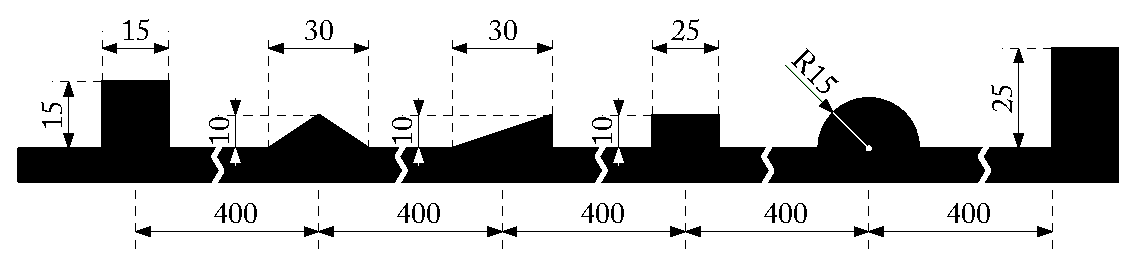
\includegraphics[width=9.5cm]{./figures/appendix_2/steps_ipe}\\[0.1in]
  \includetikz{figures/appendix_2/steps.tex}
  \caption{Quasi-static simulations of a 205/60R15 tire rolling over a stepped road surface. The \TMEasy{} model output does not change with the vertical load $F_z$ and is reported with a single line. \emph{Colors legend}: {\color{mycolor1}$\blacksquare$}~$F_z =$ \SSI{2}{\kilo\newton}, {\color{mycolor2}$\blacksquare$}~$F_z =$ \SSI{4}{\kilo\newton}, and {\color{mycolor3}$\blacksquare$}~$F_z =$ \SSI{6}{\kilo\newton}. \emph{Lines legend}: \raisebox{1.0pt}{\textbf{---}}~\Enve{}, \raisebox{1.0pt}{\textbf{--~--}}~\Swift{}, and {\color{mycolor5}$\blacksquare$}~\TMEasy{}, and {\color{black}$\blacksquare$}~road surface cross-section.}
  \label{app2:fig:steps}
\end{figure}

\begin{figure}[!htb]
  \centering
  \includetikz{figures/appendix_2/cobblestone.tex}
  \caption{Quasi-static simulations of a 205/60R15 tire rolling over a Belgian block road surface. The \TMEasy{} model output does not change with the vertical load $F_z$ and is reported with a single line. \emph{Colors legend}: {\color{mycolor1}$\blacksquare$}~$F_z =$ \SSI{2}{\kilo\newton}, {\color{mycolor2}$\blacksquare$}~$F_z =$ \SSI{4}{\kilo\newton}, and {\color{mycolor3}$\blacksquare$}~$F_z =$ \SSI{6}{\kilo\newton}. \emph{Lines legend}: \raisebox{1.0pt}{\textbf{---}}~\Enve{}, \raisebox{1.0pt}{\textbf{--~--}}~\Swift{}, and {\color{mycolor5}$\blacksquare$}~\TMEasy{}, and {\color{black}$\blacksquare$}~road surface cross-section.}
  \label{app2:fig:cobblestone}
\end{figure}

% % % % % % % % % % % % % % % % % % % % % % % % % % % % % % % % % % % % % % % %

\subsection{Full-Vehicle Model Simulation}
\label{app2:sec:simulator}

To evaluate the behavior of the presented tire-ground enveloping model in a typical use case, it is integrated into a complete \ac{RT} vehicle simulation framework, and compared with the \Swift{}~\cite{schmeitz2004semiempirical} and \TMEasy~\cite{rill2013tmeasy, rill2018sophisticated}{} enveloping models. The used framework consists of a DIL/SIL/HIL simulator based on a custom high-fidelity vehicle model. Vehicle dynamics is described by a 14 \acp{DOF} full-vehicle model able to accurately simulate the impact of suspension kinematics and compliance on vehicle behavior within the typical range of frequencies for the ride and handling analysis. Contrary to widespread practice, the vehicle dynamic equations are not linearized. This improves model accuracy in non-linear regions and vehicle attitude even in abnormal conditions. The described formulation enables the vehicle model for 3D road simulations. It is worth noting that additional \acp{DOF} are used to describe internal components' dynamics, such as the powertrain, the steering system or the tire subsystems. The structure of the model is organized in a modular fashion mirroring the mechanical interfaces of vehicle components. This modular structure makes the integration of third-party software or, more generally, of any external system a fairly straightforward process. As a result, it is possible to easily configure the vehicle model for HIL, SIL and/or DIL simulations. The developed enveloping model is thus interfaced, as a subsystem with the vehicle\ac{MB} system through a pre-defined model interface. Inputs of the tire-ground contact subsystem are the wheels' reference frames as well as the wheels' geometrical characteristics and the 3D road surface mesh. The outputs of the subsystem are, for each wheel, the equivalent tire contact point, the local contact plane, the contact penetration and the local friction coefficient. Road contact parameters, extracted from the tire-ground enveloping model, are then used by the \ac{MF}~6.2 tire model to compute contact forces.

The modeled vehicle is a passenger car with sedan-like characteristics. The vehicle features a fully electric powertrain with a front-wheel drive transmission layout. The modeled suspensions are a MacPherson configuration for the front suspensions and a Multi-Link scheme for the rear suspensions. For the sake of brevity, only the most relevant vehicle parameters are listed in \tablename~\ref{app2:tab:vehicle_data}.

\begin{table}[!htb]
  \centering
  \begin{tabular}{lc}
    \toprule
    \textbf{Parameter description}              & \textbf{Value} \\
    \midrule
    Total mass of the vehicle                   & \SSI{1300}{\kilo\gram} \\
    Center-of-mass height                       & \SSI{0.30}{\meter} \\
    Front axle distance from the center-of-mass & \SSI{1.25}{\meter} \\
    Rear axle distance from the center-of-mass  & \SSI{1.45}{\meter} \\
    Wheelbase                                   & \SSI{2.70}{\meter} \\
    Yaw inertia                                 & \SSI{1400}{\kilo\gram\meter\squared} \\
    Track width                                 & \SSI{1.50}{\meter} \\
    Steering ratio                              & \num{20} \\
    Maximum torque at wheel                     & \SSI{1200}{\newton\meter} \\
    Maximum motor power                         & \SSI{150}{\kilo\watt} \\
    Wheel inertia around rotation axis          & \SSI{1.40}{\kilo\gram\meter\squared} \\
    Size specification of the tires             & \num{205}/\num{60}R\num{15} \\
    Spring stiffness at wheel                   & \SSI{3530}{\kilo\newton\per\meter} \\
    Damping coefficients at wheel for jounce    & \SSI{789}{\newton\second\per\meter} \\
    Damping coefficients at wheel for rebound   & \SSI{1578}{\newton\second\per\meter} \\
    \bottomrule
  \end{tabular}
  \caption{Main parameters of the modeled vehicle.}
  \label{app2:tab:vehicle_data}
\end{table}

\begin{figure}[!htb]
  \centering
  \includetikz{figures/appendix_2/accelerations.tex}
  \caption{Chassis accelerations of the full-vehicle model driving over a \SSI{45}{\deg} oblique step of \SSI{1}{\centi\meter} at a longitudinal speed of \SSI{10}{\kilo\meter\per\hour}. \emph{Legend}:
  {\color{mycolor1}$\blacksquare$}~\Enve{}, {\color{mycolor2}$\blacksquare$}~\Swift{}, and {\color{mycolor3}$\blacksquare$}~\TMEasy{}.}
  \label{app2:fig:accelerations}
\end{figure}

\begin{figure}[!htb]
  \centering
  \includetikz{figures/appendix_2/forces.tex}
  \caption{Front-left tire forces of the full-vehicle model driving over a \SSI{45}{\deg} oblique step of \SSI{1}{\centi\meter} at a longitudinal speed of \SSI{10}{\kilo\meter\per\hour}. \emph{Legend}: {\color{mycolor1}$\blacksquare$}~\Enve{}, {\color{mycolor2}$\blacksquare$}~\Swift{}, and {\color{mycolor3}$\blacksquare$}~\TMEasy{}.}
  \label{app2:fig:forces}
\end{figure}

\begin{figure}[!htb]
  \centering
  \includetikz{figures/appendix_2/rhos.tex}
  \caption{Tires deflections of the full-vehicle model driving over a \SSI{45}{\deg} oblique step of \SSI{1}{\centi\meter} at a longitudinal speed of \SSI{10}{\kilo\meter\per\hour}. \emph{Legend}: {\color{mycolor1}$\blacksquare$}~\Enve{}, {\color{mycolor2}$\blacksquare$}~\Swift{}, and {\color{mycolor3}$\blacksquare$}~\TMEasy{}.}
  \label{app2:fig:rho}
\end{figure}

Model accuracy and robustness are widely tested with DIL simulations by driving the vehicle in urban scenarios, characterized by speed bumps, sidewalks or, generally, uneven road surfaces. In this work, we present the results obtained by driving the vehicle at a longitudinal speed of \SSI{10}{\kilo\meter\per\hour} over a \SSI{45}{\deg} oblique and \SSI{1}{\centi\meter} high step. The reported results are the chassis accelerations (\figurename{}~\ref{app2:fig:accelerations}), front-left tire forces (\figurename{}~\ref{app2:fig:forces}), and the tires deflections (\figurename{}~\ref{app2:fig:rho}). Note that \Enve{} and \Swift{} enveloping models present a similar behavior even in the case of a simulation of a full-vehicle model. In fact, the generated chassis accelerations, the tires' forces, and deflections are in agreement with each other. The discontinuities in both the contact point height and the banking and forward slope angles of the \TMEasy{} model reflect on the full-vehicle model simulations with abrupt changes contact forces as well as chassis acceleration not seen in experimental measurements. Notice that according to the results reported in \figurename{}~\ref{app2:fig:cobblestone}, the \Enve{} model is able to correctly estimate the contact point height, but it slightly underestimates the banking angle. This causes the correct prediction of the vertical contact force magnitude, but a slight underestimation of the lateral contact force magnitude. This error may be emphasized or reduced depending on the tire's properties.

\subsection{Real-Time Performance}
\label{app2:sec:performance}

To access the computations' performance of the \Enve{} \cpp{} software implementation, we will make use of the\ac{RTF} metric. Specifically, the \ac{RTF} is defined as the ratio between the time needed to process the input and the input duration. In order to consider a system a \ac{RT} system, \ac{RTF} should be $\leq$\,1. We performed a test in which the triangles inside the \Aabb{} of the tire are increased from 1 up to 10\textsuperscript{4}, while the number of ribs is increased from 1 to 10. The simulation platform is an iHawk\textsuperscript{TM} Concurrent Real-Time provided with \SSI{2.5}{\giga\hertz} Intel Xeon Silver 4215 8 Core, \SSI{11}{\mega\byte} cache, \SSI{32}{\giga\byte} DDR4 \ac{RAM}, and \SSI{64}{\bit} RedHawk Linux RTOS with CentoOS distribution. All tests are performed on a shielded CPU. The results reported in~\figurename{}~\ref{app2:fig:rtf_enve}, show that the \ac{RTF} of \Enve{} is mostly impacted by the number of triangles inside the \Aabb{} of the tire rather than the number of ribs. Overall, the \ac{RTF} of the software is $\leq$\,1 for a number of triangles inside the \Aabb{} of the tire up to $\approx$\,1000, which corresponds to a regular grid discretization of $\approx$\,\SSI{1.5}{\centi\meter} spacing. However, in a typical vehicle simulation, only a part of the time step can be used to perform the tire-ground contact calculations. The available time depends on several factors, such as the complexity of both the vehicle and the tire models. To the author' knowledge, a good practice is to use roughly 25\% of the integration time step to establish the contact parameters. This means that the \ac{RTF} of the software should be $\leq$\,0.25 to be considered \ac{RT}. In this case, the maximum number of triangles inside the tire \Aabb{} drops to $\approx$\,200, which corresponds to a regular grid discretization of $\approx$\,\SSI{3.5}{\centi\meter} spacing. Overall, these performances are more than sufficient for most \ac{RT} applications. Further improvements can be achieved by parallelizing the \AabbTree{}-\Aabb{} and the \Rib{}-\TriangleGround{} intersection algorithms, which are currently implemented in a serial fashion. Moreover, different instances of \Enve{} objects can run concurrently in separated CPUs to further improve the overall performance of the full-vehicle model.

\begin{figure}[!htp]
  \centering
  \includetikz{figures/appendix_2/rtf_enve.tex}
  \caption{Real-time factor of the \Enve{} algorithm \cpp{} implementation~\cite{enve} as a function of the number of triangles in the tire \Aabb{} and the number of ribs which discretize the tire.}
  \label{app2:fig:rtf_enve}
\end{figure}

% % % % % % % % % % % % % % % % % % % % % % % % % % % % % % % % % % % % % % % %

% That's all folks!
